\begin{frame}
    \centering
    \begin{figure}[H]
        
\includegraphics[keepaspectratio, width=0.7\paperwidth, height=\paperheight]{LeeLogo}
    \end{figure}
    Informatik: Data Science und Sicherheit\\
    % \textbf{Lektion 4}/
    \emoji{face-with-monocle} \emoji{deciduous-tree}: \textbf{Graphen und Bäume (Lektion 2/2)}
\end{frame}

\begin{frame}{Wiederholung letztes Mal: Knoten und Kanten}
    Knoten und Kanten \\[.5cm]
        \begin{minipage}[c]{.35\linewidth}
        \begin{figure}[H]
            \centering
            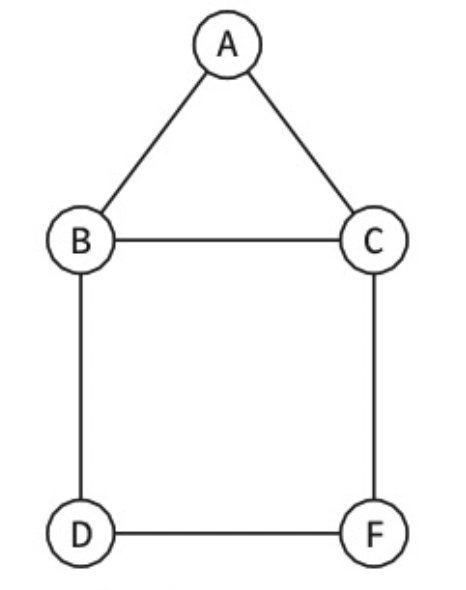
\includegraphics[keepaspectratio, width=.7\linewidth]{GrundlagenInfo/02_Graphen/Figures/4-graph.png}
        \end{figure}
        \end{minipage}
        \begin{minipage}[c]{.45\linewidth}
        \footnotesize\begin{align*}
V=&\lrc{A,B,C,D,F}\\        
E=&\{\lrc{A,B},\lrc{A,C},\lrc{B,C},\\
 &\lrc{B,D},\lrc{C,F},\lrc{D,F}\}
        \end{align*}
        \end{minipage}\normalsize    
\end{frame}

\begin{frame}{Wiederholung letztes Mal: Zusammenhängende Graphen}
        Zusammenhängende Graphen
            \begin{figure}
            \centering
            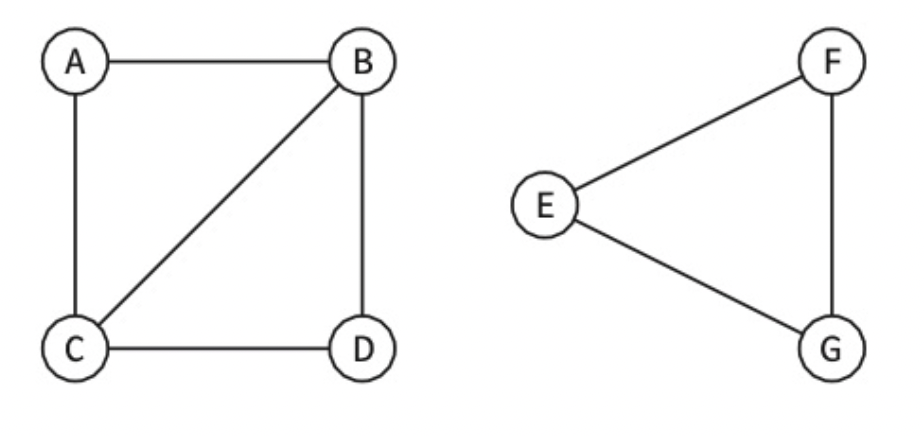
\includegraphics[keepaspectratio, width=0.35 \paperwidth]{GrundlagenInfo/02_Graphen/Figures/4-graph-zusammenhaengend.png}
        \end{figure}    
\end{frame}

\begin{frame}{Wiederholung letztes Mal: Grad eines Graphen}
    Grad eines Graphen
    \begin{itemize} 
        \item Der \textbf{Grad eines Knotens} $x \in V$, bezeichnet als $\deg(x)$, ist die Anzahl der mit x verbundenen Kanten
        \item Der \textbf{Grad eines Graphen} $G$, bezeichnet als $\deg(G)$, ist das Maximum der Grade aller Knoten im Graphen
    \end{itemize}
\end{frame}

\begin{frame}{Wiederholung letztes Mal: Vollständige Graphen}
    Vollständige Graphen   
    $$\forall x\in V:\quad \deg(x)=n-1$$
        \begin{figure}
            \centering
            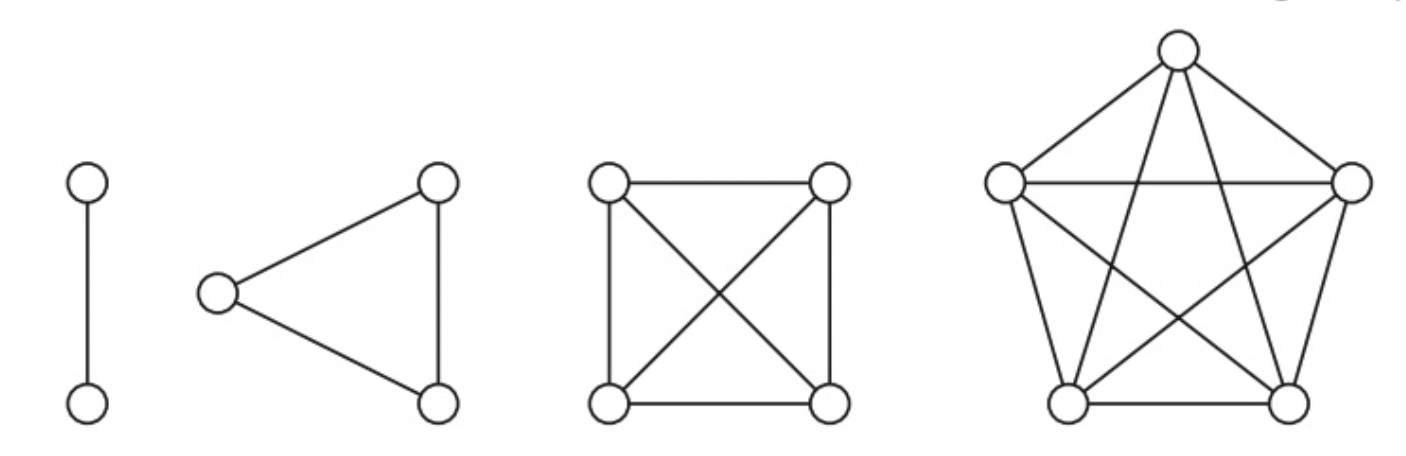
\includegraphics[keepaspectratio, width=0.45 \paperwidth]{GrundlagenInfo/02_Graphen/Figures/4-graph-vollstaendig.png}
        \end{figure}
\end{frame}

\begin{frame}{Wiederholung letztes Mal: Vollständige Graphen}
    Letztes Mal
    \begin{itemize}
        \item Wege und Kreise
        \item Hamiltonsche' und Euler'sche Wege
        \item Färben eines Graphen
    \end{itemize}
            \begin{figure}[H]
            \centering
            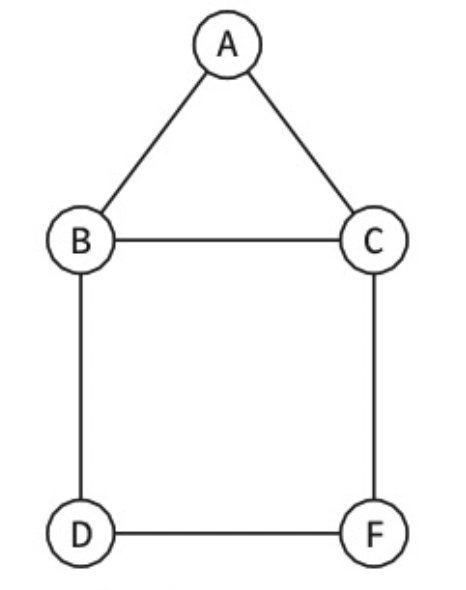
\includegraphics[keepaspectratio, width=.3\linewidth]{GrundlagenInfo/02_Graphen/Figures/4-graph.png}
        \end{figure}
    
\end{frame}

\begin{frame}{Programm}
Heute
    \begin{itemize}
        \item \emoji{zero}\emoji{one} \textbf{Binäre Darstellung} von Graphen
        \item \emoji{right-arrow} \textbf{Gerichtete} Graphen und Bäume
        \item \emoji{deciduous-tree} \textbf{Bäume}
    \end{itemize}
\end{frame}
\begin{frame}{\emoji{zero}\emoji{one} Binäre Darstellung von Graphen}
\begin{figure}[H]
    \centering
    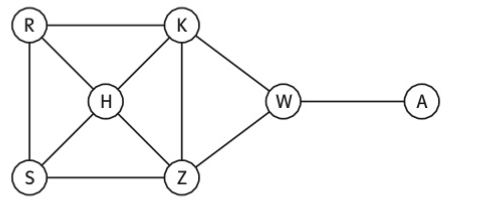
\includegraphics[keepaspectratio, width=.5\paperwidth]{GrundlagenInfo/02_Graphen/Figures/graphen-bin.png}
\end{figure}
\textbf{Nachbarschaftsmatrix} (= Tabelle) des Graphen:
\begin{table}[H]
\begin{tabular}{c||c|c|c|c|c|c|c}
  & R & S & H & K & Z & W & A \\ \midrule
R & 0 & 1 & 1 & 1 & 0 & 0 & 0\\ \hline
S & 1 & 0 & 1 & 0 & 1 & 0 & 0\\ \hline
H & 1 & 1 & 0 & 1 & 1 & 0 & 0\\ \hline
K & 1 & 0 & 1 & 0 & 1 & 1 & 0\\ \hline
Z & 0 & 1 & 1 & 1 & 0 & 1 & 0\\ \hline
W & 0 & 0 & 0 & 1 & 1 & 0 & 1\\ \hline
A & 0 & 0 & 0 & 0 & 0 & 1 & 0\\ 
\end{tabular}
\end{table}

\end{frame}

\begin{frame}{\emoji{right-arrow} Gerichtete Graphen}
\begin{figure}[H]
    \centering
    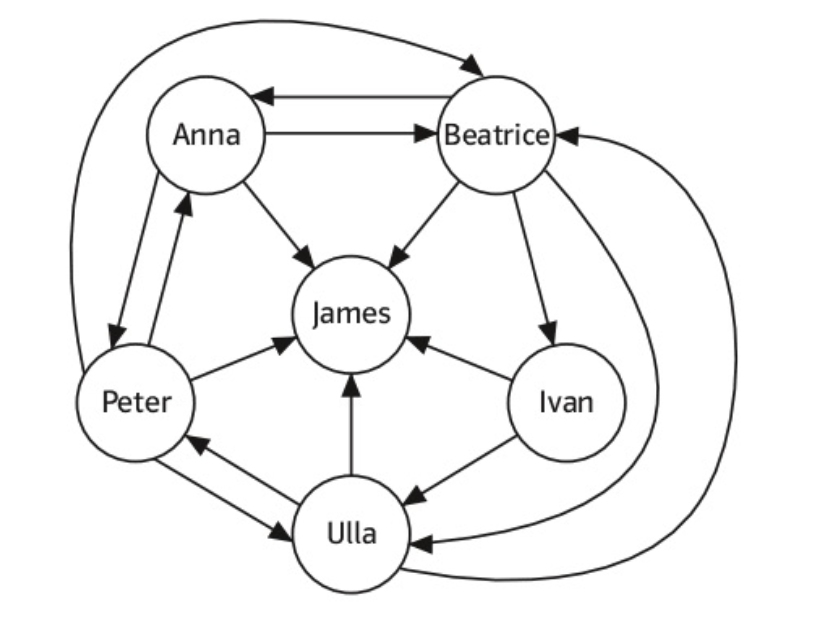
\includegraphics[keepaspectratio, width=.4\paperwidth]{GrundlagenInfo/02_Graphen/Figures/graphen-gerichtet.png}
\end{figure}
\textbf{Nachbarschaftsmatrix} (= Tabelle) des Graphen:


\end{frame}

\begin{frame}{\emoji{deciduous-tree} Ungerichtete Bäume}
Definitionen
\begin{itemize}
    \item \emoji{deciduous-tree} Ein Graph heisst \textbf{Baum}, wenn er \textbf{zusammenhängend} und \textbf{kreisfrei} ist.
    \item \emoji{maple-leaf} Knoten mit Grad 1 = \textbf{Blätter} eines Baums
\end{itemize}
\only<2->{
Welche dieser drei Graphen sind Bäume? Weshalb (nicht)?
\begin{figure}[H]
    \centering
    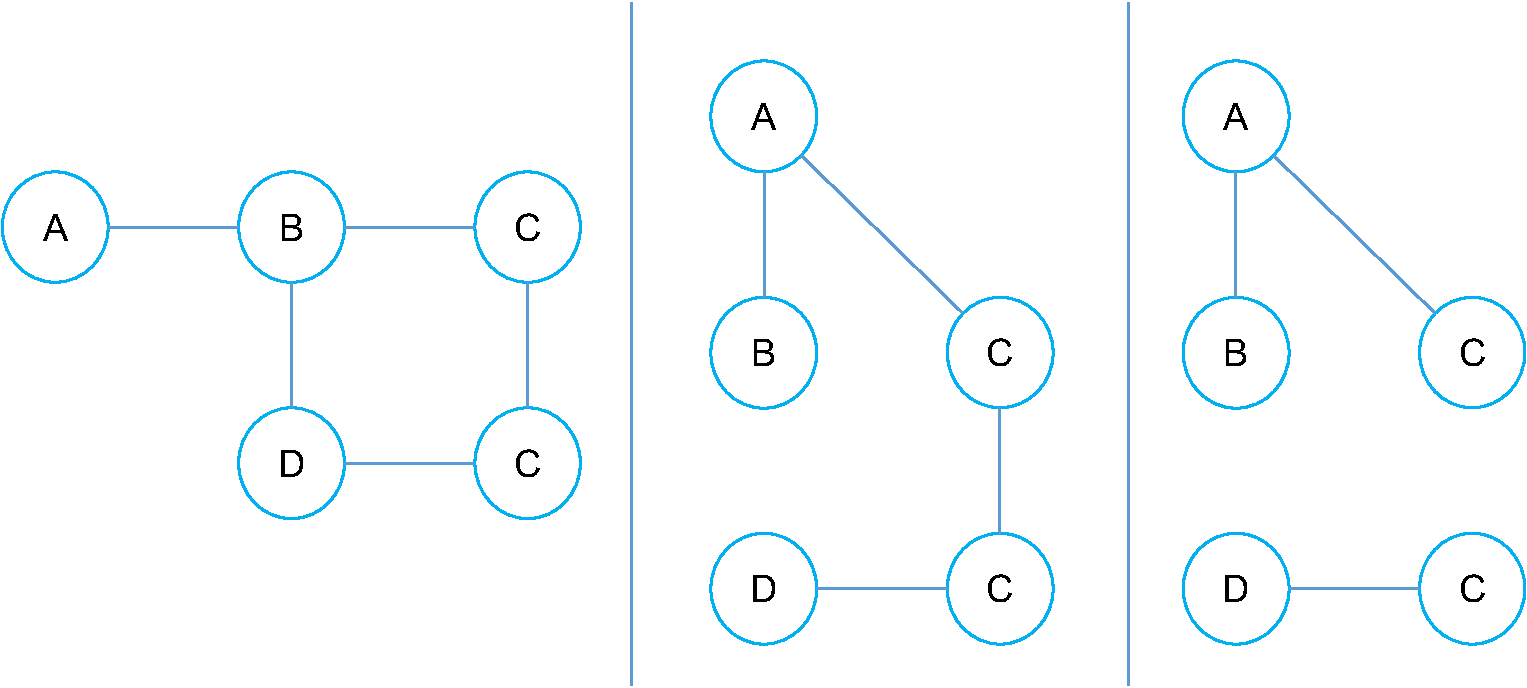
\includegraphics[keepaspectratio, width=.8\linewidth]{GrundlagenInfo/02_Graphen/Figures/graphen-baeume.pdf}
\end{figure}
}
\only<3>{$\rightarrow$ S. 38, neue Konzepte und Begriffe}
\end{frame}

\begin{frame}{\emoji{deciduous-tree} Gerichtete Bäume}
    \begin{figure}[H]
    \centering
    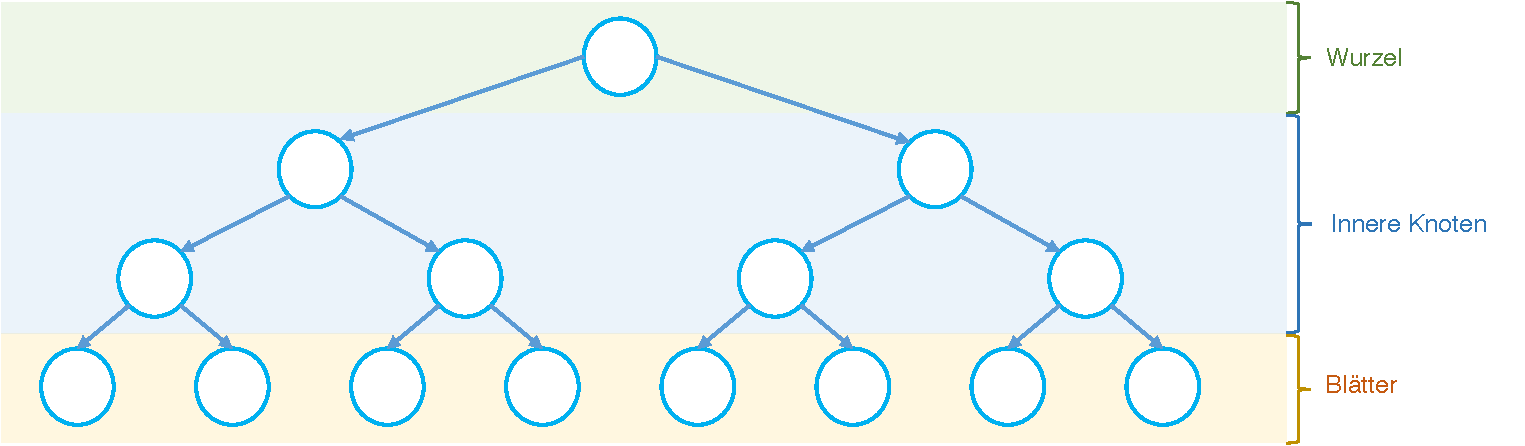
\includegraphics[keepaspectratio, width=\linewidth]{GrundlagenInfo/02_Graphen/Figures/binary-tree.pdf}
\end{figure}
\begin{itemize}[<+->]
    \item \textbf{Wurzel} = Knoten mit Eingangs-Grad 0
    \item \emoji{maple-leaf} \textbf{Blätter} = Knoten mit Ausgangs-Grad 0
    \item \textbf{Innere Knoten} = Alle anderen Knoten (weder Blätter noch Wurzel)
    \item Das Beispiel oben ist ein \textbf{gewurzelter Baum}: Es gibt eine einzige Wurzel, von der aus alle Knoten über gerichtete Kanten erreichbar sind
\end{itemize}
\end{frame}

\begin{frame}{Auftrag}
\begin{itemize}
    \item Aufgabe 1.50
    \item Aufgabe 1.51    
    \item Aufgabe 1.54
    \item Aufgabe 1.58
    \item Aufgabe 1.62
    \item \textbf{Challenge}: 
    \begin{itemize}
        \item Aufgabe 1.59 (+ Lösung lesen), 1.61
        \item Aufgabe 1.63
    \end{itemize}
\end{itemize}
\end{frame}